\begin{figure}
    \begin{center}
    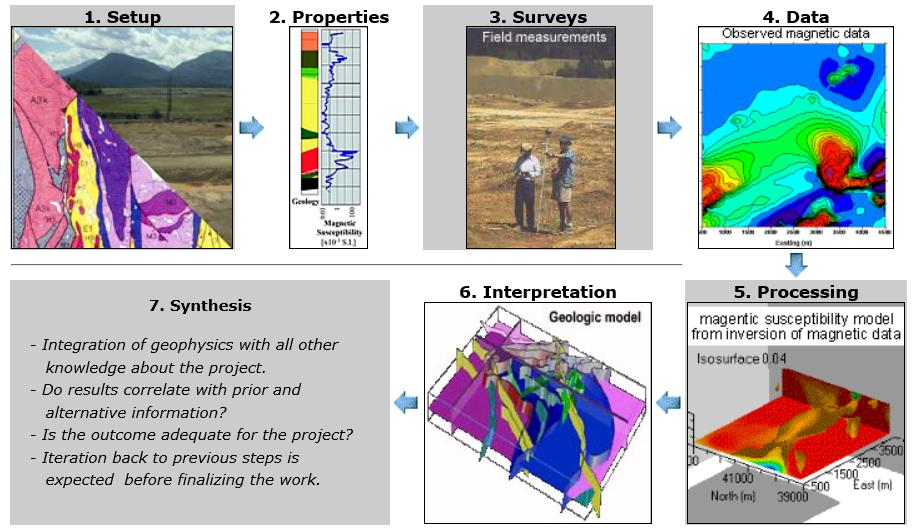
\includegraphics[width=0.8\textwidth]{figures/education/seven_steps.jpg}
    \end{center}
\caption{
   Seven step framework used for the case histories in \href{https://em.geosci.xyz}{https://em.geosci.xyz}.
   (1) Setup: describe the geoscientific question and objectives that are to be addressed.
   (2) Properties: identify the diagnostic physical properties (e.g. density, electrical conductivity, magnetic susceptibility, etc.).
   (3) Survey: design a survey that is suitable for detecting the physical property contrasts relevant to the application.
   (4) Data: carry out the field survey and collect the data set(s).
   (5) Processing: plot the data and apply the analysis steps needed to interpret the data (e.g. invert the data).
   (6) Interpretation: interpret the results in terms of the identified physical properties and original geoscience objective.
   (7) Synthesis: integrate the interpretation with geologic and other information relevant to the application in order to address the original geoscience objective.
   This image and caption are adapted from:
   \href{https://em.geosci.xyz/content/geophysical_surveys/fundamentals/seven_steps.html}{https://em.geosci.xyz/content/geophysical\_surveys/fundamentals/ seven\_steps.html}
}
\label{fig:seven_steps}
\end{figure}



